\section{Experimental protocols and complete condition-level results}\label{app:experiments}
All data are generated within the release. The raw CSVs include failed or unfavorable comparisons as well as favorable ones. The theoretical family uses a unit-norm bisector error; its numbers should not be confused with unnormalized illustrative examples. Population linear risk is $\norm{\theta-\theta^*}^2/2$ under identity target covariance.

\subsection{Exact and robustness suites}
The exact family sweep uses source angles $15,30,45,60,75$ degrees; orthogonal masses $0,10^{-6},10^{-4},10^{-2},1$; ridges $0,0.05$; and 61 budgets between $\max\{1,\tau\}$ and 16. The static audit uses five angles, four masses, two ridges, and five budgets, comparing the analytic optimum to 101 weights spanning $[0,1]$. Its numerical grid is an audit, not the source of the optimality claim.

The isotropic suite draws 160 independent pairs of Wishart-like PSD matrices, with dimensions cycling through 2, 4, 8, and 12. Durations are uniform on $[0.02,3]$, and phase weights are uniform on $[0,1]$. The full-rank bound suite draws 400 two-phase schedules with angles in $[0.1,1.5]$ radians, log-uniform masses in $[10^{-6},1]$, ridges in $[0,0.2]$, and budgets in $[0.1,25]$. The code records absolute inequality margins, not an arbitrarily rounded success flag.

Perturbation tests independently rotate both source vectors and the initial vector by Gaussian angles with standard deviation $0$, $0.001$, $0.01$, $0.05$, or $0.1$ radians. Each condition has 24 seeds at budgets 4 and 8. The schedule retains the nominal $45^\circ$ preparation time. The static comparator uses a 257-point grid followed by a bounded scalar refinement near its best grid point, and is labeled a numerical comparator rather than a certified global optimum for perturbed inputs. The aggregate results are in Table~\ref{tab:perturb}.

\begin{table}[h]
\centering\small
\caption{Perturbed geometry: preparation gain against the numerical static comparator.}\label{tab:perturb}
\begin{tabular}{rrrrr}\toprule
Budget & Angular standard deviation & Median gain & Wins & Cases\\\midrule
4 & 0 & 1.8904 & 24 & 24 \\
4 & 0.001 & 1.8880 & 24 & 24 \\
4 & 0.01 & 1.7313 & 24 & 24 \\
4 & 0.05 & 0.6871 & 10 & 24 \\
4 & 0.1 & 0.2109 & 4 & 24 \\
8 & 0 & 6.1003 & 24 & 24 \\
8 & 0.001 & 2.0728 & 16 & 24 \\
8 & 0.01 & 0.0336 & 5 & 24 \\
8 & 0.05 & 0.0014 & 1 & 24 \\
8 & 0.1 & 0.0003 & 0 & 24 \\
\bottomrule\end{tabular}
\end{table}

The Euler check uses step sizes $0.2,0.1,0.05,0.025,0.0125$, budgets 2, 4, 8, and ridge 0.05. The switch is rounded to the nearest step for \emph{both} exact flow and Euler dynamics. Thus the measured operator discrepancy tests Lemma~\ref{lem:euler}, not an unaccounted switch-time error.

\begin{figure}[t]
\centering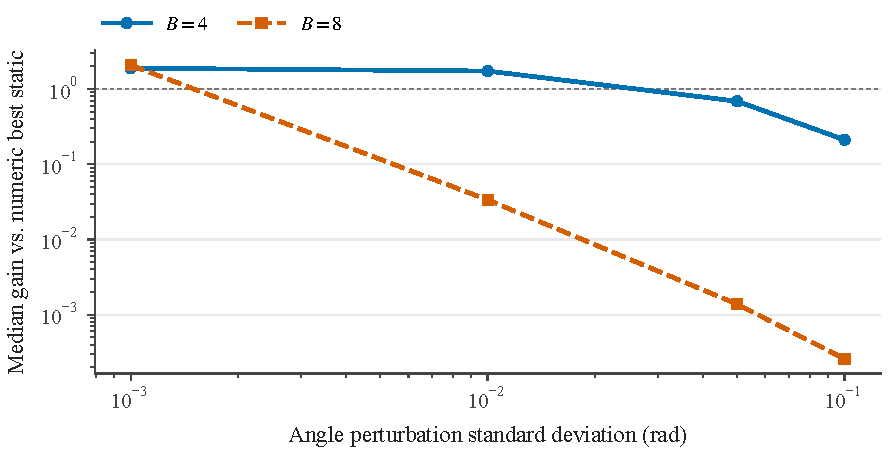
\includegraphics[width=.92\linewidth]{figures/geometry_robustness.pdf}
\caption{Sensitivity of the nominal preparation schedule. There are 24 independent perturbations per point. The long-budget gain is much more sensitive to small rotations. A value below one means preparation is worse.}\label{fig:robust}
\end{figure}

\subsection{Spectral and capacity experiments}
Each block is the $45^\circ$ family, with source scales $\lambda_j=j^{-1}$ and normalized initial masses proportional to $j^{-1-\beta}$ for $\beta\in\{0.5,1,2\}$. Ridge is 0 or 0.1 within the base block, and is scaled together with the block. There are 2,048 trained blocks and budgets 4, 16, 64, 256. The entire tail beyond the trained blocks is included using the Hurwitz zeta function. The balanced mixture is analytically best among all static weights because it is best in each block separately.

A two-phase candidate is parameterized by $(p_1,p_2,f)\in[0,1]^3$, with durations $fB$ and $(1-f)B$. A local L-BFGS-B search uses six starting points: $(0.5,0.5,0.5)$, $(1,0,0.15)$, $(1,0,0.5)$, $(0.9,0.1,0.3)$, $(0.8,0.1,0.7)$, and $(0.9,0.3,0.5)$. Its maximum iteration and function-call budgets are 80 and 500, with function tolerance $10^{-11}$ and gradient tolerance $10^{-10}$. The static candidate is always included. This procedure does not certify a global two-phase optimum. It only asks whether a small numerical search finds a substantial shared-schedule improvement.

The capacity experiment uses $(\alpha,\beta)=(1,1),(1,2),(2,1)$, 26 total-work budgets logarithmically spaced between $10^2$ and $10^7$, and a fixed list of capacities obtained by rounding 97 logarithmically spaced values between 2 and 32,768 and removing duplicates. For each capacity, $B=C/J$ and the balanced static risk is exact. Slopes fit the final ten budget points by least squares in log coordinates. Capacity selection is over this grid, whereas the theorem concerns all integer capacities; the slope check is not a global finite-budget capacity certificate.

\begin{figure}[t]
\centering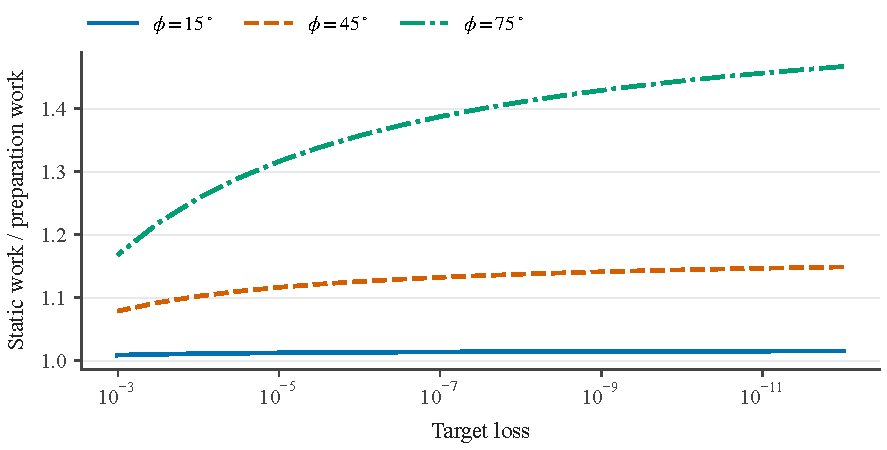
\includegraphics[width=.92\linewidth]{figures/work_savings.pdf}
\caption{Exact compute-to-target ratios for the known-direction construction. Even where the equal-work loss ratio diverges, the work ratio approaches the finite limit $1/a$ at zero ridge. The asymptotic regime is approached slowly for nearly orthogonal sources because preparation is expensive.}\label{fig:work}
\end{figure}

\subsection{Pilot and planning-cost experiment}
The known source angle is $45^\circ$ with no ridge. True unit residual directions are the bisector plus nine offsets equally spaced between $-0.06$ and $0.06$ radians. For each total budget $B\in\{4,8\}$, coordinate noise $\sigma\in\{0.05,0.2\}$, sample count per coordinate $n\in\{64,256,1024\}$, and query price $q\in\{10^{-4},10^{-3}\}$, we run 90 observations cycling over the nine true directions. We compare planning charges $h=0$ and $h=0.02$ using identical observation draws. There are 2,160 cases per charge, 4,320 rows total. The confidence level is $1-\delta=0.95$; the conservative Gaussian radius covers 2,158 cases for each charge.

The remaining training budget is exactly $B-2nq-h$. Both the $A$-then-$B$ and $B$-then-$A$ preparation schedules are evaluated at that remaining budget. The smaller risk upper bound chooses the candidate. The full-budget static lower envelope uses 2,048 cells at $B=4$ and 8,192 cells at $B=8$. On rejection, a static weight minimizing estimated-state risk over 512 cell centers is trained with the remaining budget. For descriptive gain and false-acceptance checks, a separate 1,025-point static grid with local refinement evaluates the true residual at the original budget. The certificate itself does not use this hidden reference value.

\begin{table}[h]
\centering\small
\caption{Pilot cost matters even when accepted decisions are correct. Medians use static risk divided by selected risk.}\label{tab:pilot}
\begin{tabular}{rrrrr}\toprule
Planning charge & Accepts / cases & False accepts & Accepted median & All-case median\\\midrule
0 & 25 / 2,160 & 0 & 1.447 & 0.417\\
0.02 & 23 / 2,160 & 0 & 1.400 & 0.403\\
\bottomrule\end{tabular}
\end{table}

The prices $q$ and $h$ are declared cost-model parameters. We do not infer them from processor clocks, nor claim that $h=0.02$ is the actual cost of every planner implementation. A real application must calibrate these prices and also decide whether to run the pilot. Neither a zero false-acceptance count nor a correct conditional theorem makes that initial purchase automatically beneficial.

\subsection{Finite-data linear training}
For each source, draw $x\sim N(0,G_i)$ and $y=x^\top\theta^*+\xi$, where $\theta^*=-u$ and $\xi\sim N(0,\sigma_y^2)$. Both source covariances include ridge $0.02$. Each source provides a cached dataset of $n\in\{128,1024\}$ samples. Source angles are 45 and 70 degrees; label standard deviation is 0 or 0.1; normalized budgets are 4 or 8. These are 16 settings, with 20 independent training/data seeds each.

SGD starts at zero, uses step size 0.025 and batch size 32, and draws with replacement from the cached source datasets. The static weight is implemented as the probability that each batch position uses source $A$. Within a seed, all methods share datasets, indices, and uniform mixture draws. The explicit preparation time is rounded to a step boundary. There are 11 static probabilities $0,0.1,\ldots,1$, both preparation orders, an exposure-matched static probability, and a greedy oracle choosing the source with larger current population quadratic decrease. Every trained run uses the same number of gradient examples at a fixed budget.

The principal comparator takes the minimum target risk over the 11 static weights separately for each realized seed. This is a stronger benchmark than selecting a weight on independent validation data, and its tuning cost is not charged. It is not a proposed deployable algorithm. This choice makes positive comparisons more demanding, but also means an average gain below one does not show that no practical schedule could help. All method-level risks, including the greedy and exposure-matched baselines, are retained in the raw CSV.

\begin{table}[h]
\centering\small
\caption{Preparation versus hindsight static grid in all 16 linear settings. Intervals are paired percentile bootstrap intervals for the median gain across 20 seeds.}\label{tab:linear}
\begin{tabular}{rrrrrr}\toprule
Angle & Noise & Samples/source & Budget & Median [95\% interval] & Wins\\\midrule
45 & 0 & 128 & 4 & 0.863 [0.662, 1.432] & 9/20 \\
45 & 0 & 128 & 8 & 0.104 [0.060, 0.286] & 4/20 \\
45 & 0 & 1024 & 4 & 1.513 [1.268, 1.637] & 18/20 \\
45 & 0 & 1024 & 8 & 0.192 [0.059, 0.334] & 2/20 \\
45 & 0.1 & 128 & 4 & 0.913 [0.518, 1.141] & 8/20 \\
45 & 0.1 & 128 & 8 & 0.130 [0.084, 0.319] & 3/20 \\
45 & 0.1 & 1024 & 4 & 1.569 [1.248, 1.813] & 17/20 \\
45 & 0.1 & 1024 & 8 & 0.294 [0.123, 0.681] & 4/20 \\
70 & 0 & 128 & 4 & 1.665 [1.290, 2.018] & 19/20 \\
70 & 0 & 128 & 8 & 0.095 [0.020, 0.286] & 3/20 \\
70 & 0 & 1024 & 4 & 2.582 [2.081, 2.750] & 20/20 \\
70 & 0 & 1024 & 8 & 0.519 [0.104, 2.176] & 7/20 \\
70 & 0.1 & 128 & 4 & 1.841 [1.297, 2.232] & 17/20 \\
70 & 0.1 & 128 & 8 & 0.208 [0.169, 0.508] & 3/20 \\
70 & 0.1 & 1024 & 4 & 2.285 [1.955, 2.443] & 20/20 \\
70 & 0.1 & 1024 & 8 & 0.388 [0.199, 0.998] & 5/20 \\
\bottomrule\end{tabular}
\end{table}

\subsection{Fully trained nonlinear stress test}
The source distributions have angle $45^\circ$ and ridge $0.05$. Each cached source has 512 examples; the teacher remains linear. A two-layer network
\[
 f(x)=v^\top\tanh(Wx+b)+c
\]
has input dimension two and width 16. Hidden weights are initialized independently from $N(0,0.5^2)$, output weights and biases are zero, and all parameters are updated by SGD. The learning rate is 0.02, batch size is 32, and training lasts 200 or 800 steps, with label standard deviation 0 or 0.1. The test set contains 4,096 independent standard-Gaussian inputs and noiseless teacher labels, fixed across methods.

For this stress test, the linear-model switch \emph{fraction} is transferred using reference budgets 4 and 8 for the 200- and 800-step settings respectively. In particular, 800 neural steps times learning rate 0.02 is not claimed to equal reference budget 8 or to implement the quadratic flow. The budget for neural comparisons is the actual number of steps and processed examples. This is a heuristic schedule-transfer experiment, not a test that a nonlinear Hessian obeys the theorem. Five static probabilities, both preparation orders, and the exposure-matched static probability use the same initialization and stochastic draws within each seed. There are 12 independent seeds per setting. A finite-difference unit test independently checks the manual backpropagation equations.

\begin{table}[h]
\centering\small
\caption{All nonlinear conditions. No condition has a median gain above one.}\label{tab:nonlinear}
\begin{tabular}{rrrr}\toprule
Label noise & Training steps & Median gain [95\% interval] & Wins / 12\\\midrule
0 & 200 & 0.925 [0.677, 1.058] & 5/12 \\
0 & 800 & 0.895 [0.784, 0.997] & 3/12 \\
0.1 & 200 & 0.901 [0.824, 0.981] & 2/12 \\
0.1 & 800 & 0.863 [0.782, 0.928] & 1/12 \\
\bottomrule\end{tabular}
\end{table}

\begin{figure}[t]
\centering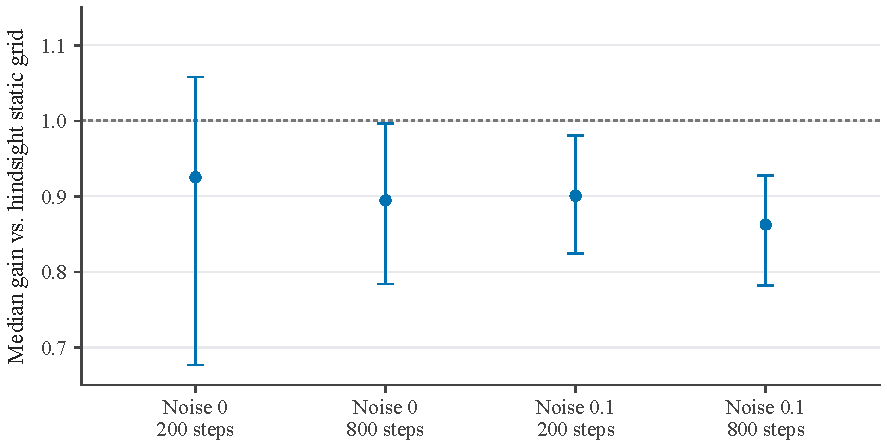
\includegraphics[width=.92\linewidth]{figures/nonlinear_gain.pdf}
\caption{The negative nonlinear stress test. Both layers learn, so this is not a fixed random-feature model. Error bars show unadjusted paired 95\% bootstrap intervals for median gain versus a per-seed hindsight static grid.}\label{fig:nonlinear}
\end{figure}

\subsection{Statistics, reproducibility, and reporting scope}
The linear and nonlinear summary intervals use 4,000 percentile-bootstrap resamples of paired gain ratios, with seed 91021. Independent units are data/training seeds, not individual examples or optimization steps. The intervals are descriptive and are not adjusted for comparisons across settings. They do not quantify uncertainty about transfer to different tasks. The exact-matrix and capacity curves are deterministic and do not need error bars. Pilot simulations are controlled scenarios, not trials sampled from a real deployment population.

The release records Python and package versions per suite, raw scientific CSVs, deterministic summary scripts, separate matplotlib figures, and an artifact integrity manifest. Scientific CSV reproducibility is checked separately from runtime metadata. Random generators use NumPy's default generator with explicit seeds. Tests include analytic family identities, Golden--Thompson comparisons, the conditioning bound, commuting controls, the two-phase lower bound, state-ball envelopes, Duhamel perturbations, independent high-precision matrix exponentials, volume bounds, spectral implementation equivalence, and neural finite differences. Passing these tests is evidence of implementation consistency, not a substitute for an independent mathematical review.

